\part[Anhang und Verzeichnise]{Anhänge und Verzeichnise
                  \begin{center}
                     \begin{minipage}[c]{10.7cm}
                        \small Hitobito: Neue Generation von Personen-Filtern \\
                        Autor: Marc Egli
                     \end{minipage}
                  \end{center}
                 }

\chapter{Verzeichnise}

\listoftables

\listoffigures

\lstlistoflistings

\renewcommand\bibname{Quellenverzeichnis}
\begin{thebibliography}{9}
    \bibitem[Agile Scrum Group - Product Owner]{Agile Scrum Group} \url{https://agilescrumgroup.de/product-owner-aufgaben/}, (14.01.2025)
    \bibitem[Agile Scrum Group - Scrum Master]{Agile Scrum Group} \url{https://agilescrumgroup.de/scrum-master-aufgaben/}, (14.01.2025)
    \bibitem[Agile Scrum Group - Entwickler]{Agile Scrum Group} \url{https://scrumguide.de/entwickler/}, (14.01.2025)
    \bibitem[StackExchange - Code Font in Latex]{StackExchange} \url{https://tex.stackexchange.com/questions/36030/how-to-make-a-single-word-look-as-some-code}, (15.01.2025)
    \bibitem[Overleaf - Lists in Latex]{Overleaf} \url{https://www.overleaf.com/learn/latex/Lists}, (15.01.2025)
    \bibitem[StackExchange - Landscape Mode Latex]{StackExchange} \url{https://tex.stackexchange.com/questions/337/how-to-change-certain-pages-into-landscape-portrait-mode}, (16.01.2025)
    \bibitem[StackOverflow - Vertical Alignment in Table Latex]{StackOverflow} \url{https://stackoverflow.com/questions/63364815/vertical-alignment-of-text-in-a-table-in-latex}, (16.01.2025)
    \bibitem[StackHawk - XSS Attacks in Rails]{StackHawk} \url{https://www.stackhawk.com/blog/rails-xss-examples-and-prevention/}, (16.01.2025)
    \bibitem[RubyGems - CanCanCan]{RubyGems} \url{https://rubygems.org/gems/cancancan/versions/3.5.0?locale=en}, (17.01.2025)
    \bibitem[StackExchange - Multicolumn in Latex]{StackExchange} \url{https://tex.stackexchange.com/questions/131867/using-multicolumn-in-latex}, (17.01.2025)
    \bibitem[Honeybadger - Enums in Rails]{Honeybadger} \url{https://www.honeybadger.io/blog/how-to-use-enum-attributes-in-ruby-on-rails/}, (21.01.2025)
    \bibitem[StackOverflow]{StackOverflow - Type of object in ruby} \url{https://stackoverflow.com/questions/15769739/determining-type-of-an-object-in-ruby}, (21.01.2025)
    \bibitem[StackOverflow - Optional Arguments]{StackOverflow} \url{https://stackoverflow.com/questions/9710303/rails-optional-argument}, (21.01.2025)
    \bibitem[StackOverflow - Passing Class]{StackOverflow} \url{https://stackoverflow.com/questions/60853529/passing-class-as-argument-in-ruby}, (21.01.2025)
    \bibitem[StackOverflow - Postgres Subquery]{StackOverflow} \url{https://stackoverflow.com/questions/12238621/sql-subquery-has-too-many-columns}, (21.01.2025)
    \bibitem[StackOverflow - Load path]{StackOverflow} \url{https://stackoverflow.com/questions/1223481/adding-a-directory-to-the-load-path-in-rails}, (21.01.2025)
\end{thebibliography}
\addcontentsline{toc}{subsection}{Quellenverzeichnis}

\chapter{Verwendete Abkürzungen}

\begin{table}[H]
    \rowcolors{2}{puzzleblue!30}{white}
    \begin{tabular}{|L{0.3\textwidth}|L{0.6\textwidth}|}
        \hline
        \rowcolor{puzzleblue} \textbf{\color{white}Abkürzung} & \textbf{\color{white}Bedeutung} \\[12pt]
        \hline
        TODO: Abkürzung & TODO: Beschreibung \\
        \hline
    \end{tabular}
    \caption{Verwendete Abkürzungen}
\end{table}

\chapter{Glossar}

\begin{table}[H]
    \rowcolors{2}{puzzleblue!30}{white}
    \begin{tabular}{|L{0.3\textwidth}|L{0.6\textwidth}|}
        \hline
        \rowcolor{puzzleblue} \textbf{\color{white}Bezeichnung} & \textbf{\color{white}Bedeutung} \\[12pt]
        \hline
        TODO: Wort & TODO: Beschreibung \\
        \hline
    \end{tabular}
    \caption{Glossar}
\end{table}

\chapter{Anhänge}

\section{Sitzungsprotokolle}

\section{Git commit convention}
\label{sec:gitconv}
\begin{figure}[h]
    \centering
    \fbox{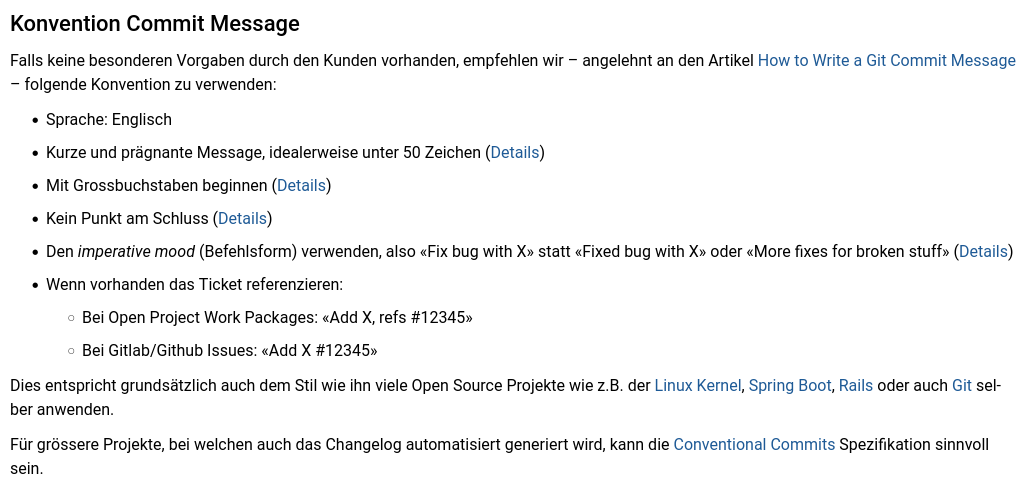
\includegraphics[width=1\textwidth,]{git_commit_conventions.png}}
    \caption{Puzzle ITC Git commit conventions}
    \end{figure}

\section{Security conventions}
\label{sec:secconv}
\begin{figure}[h]
    \centering
    \fbox{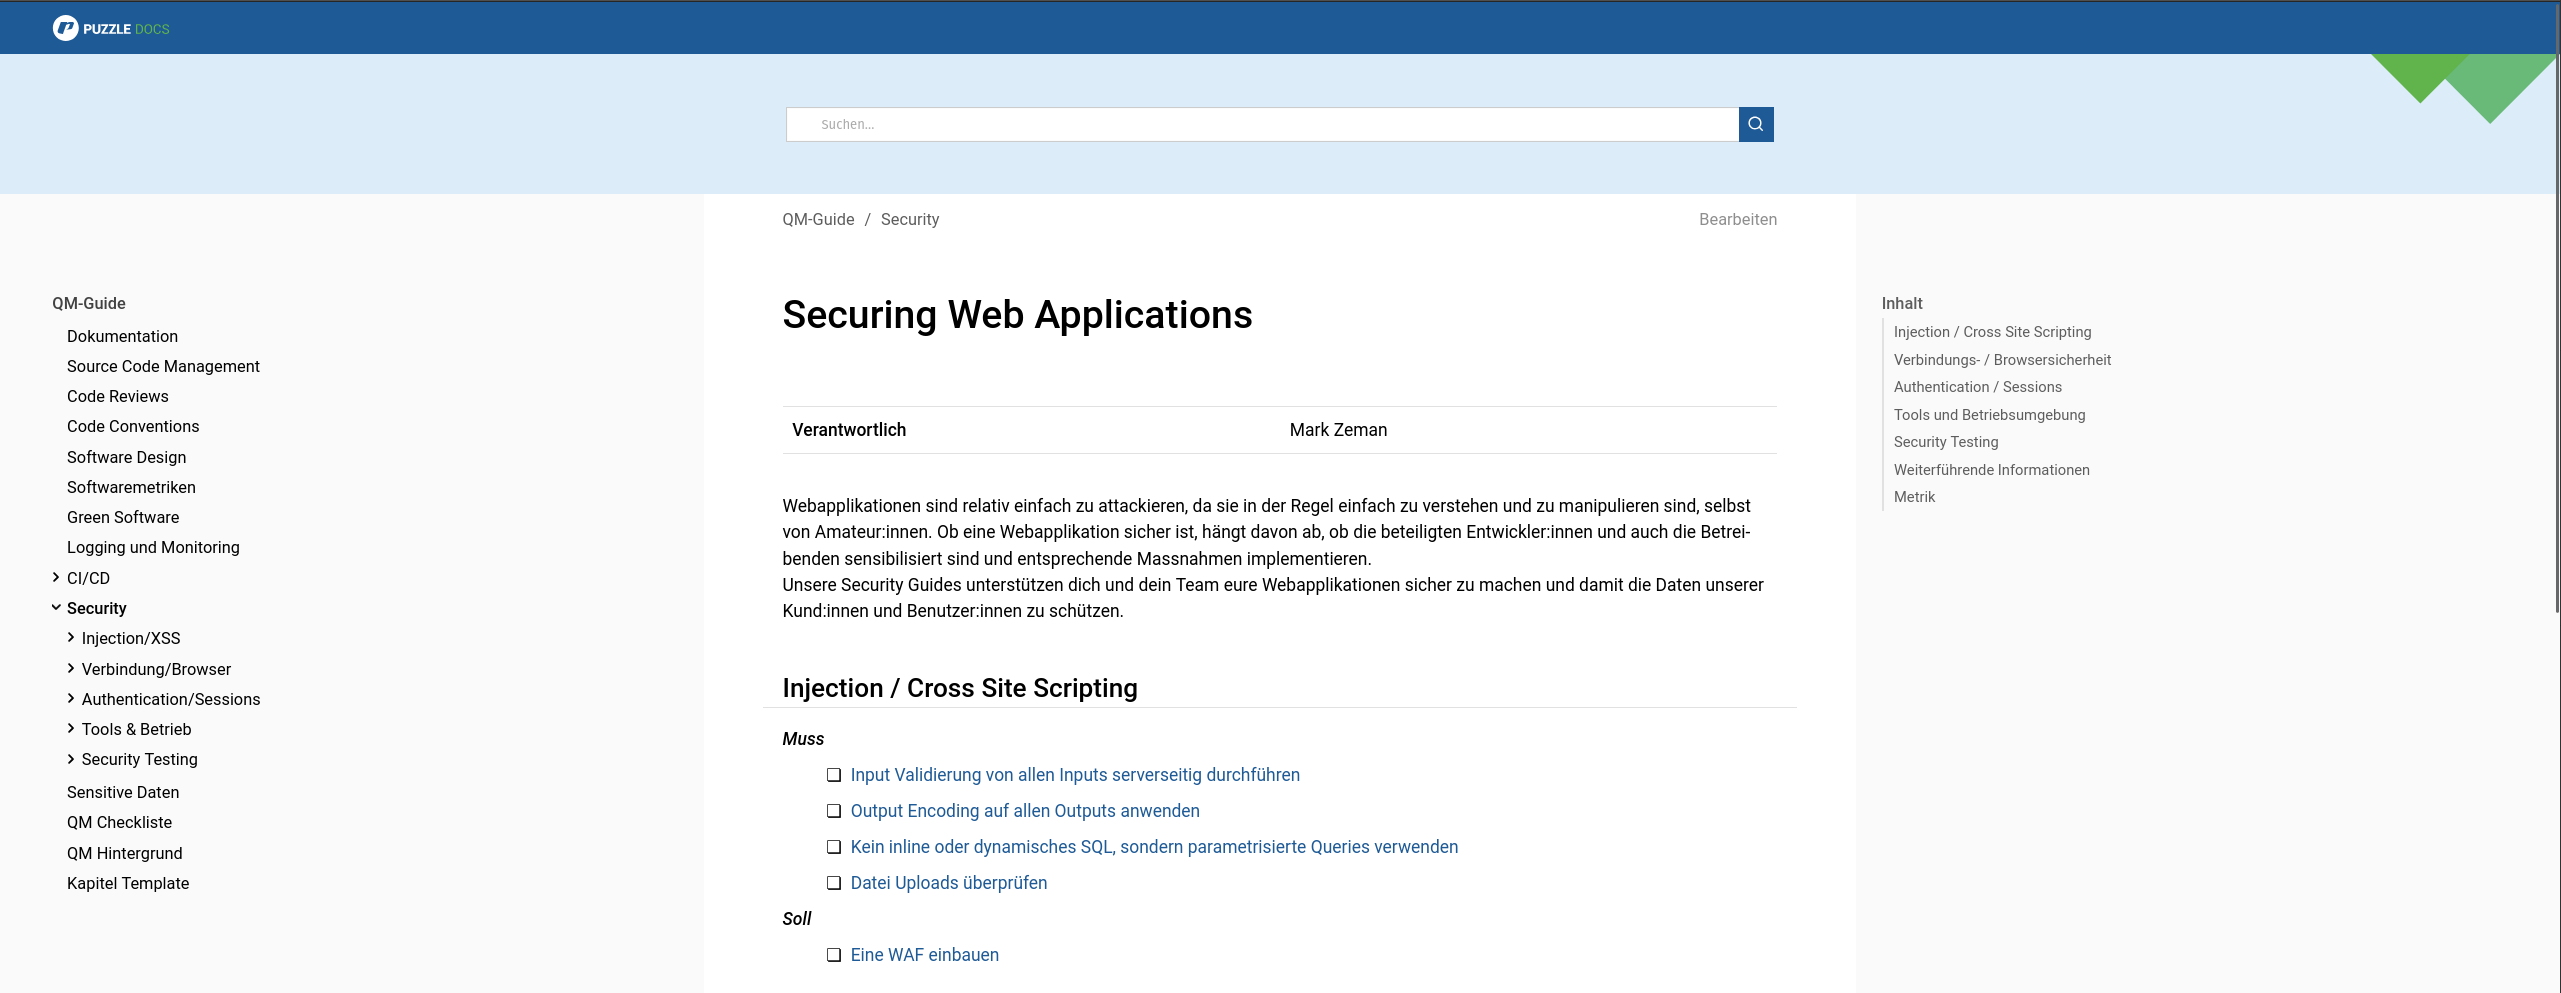
\includegraphics[width=1\textwidth,]{security_conventions_1.png}}
    \caption{Puzzle ITC security conventions 1/3}
    \end{figure}
\begin{figure}[h]
    \centering
    \fbox{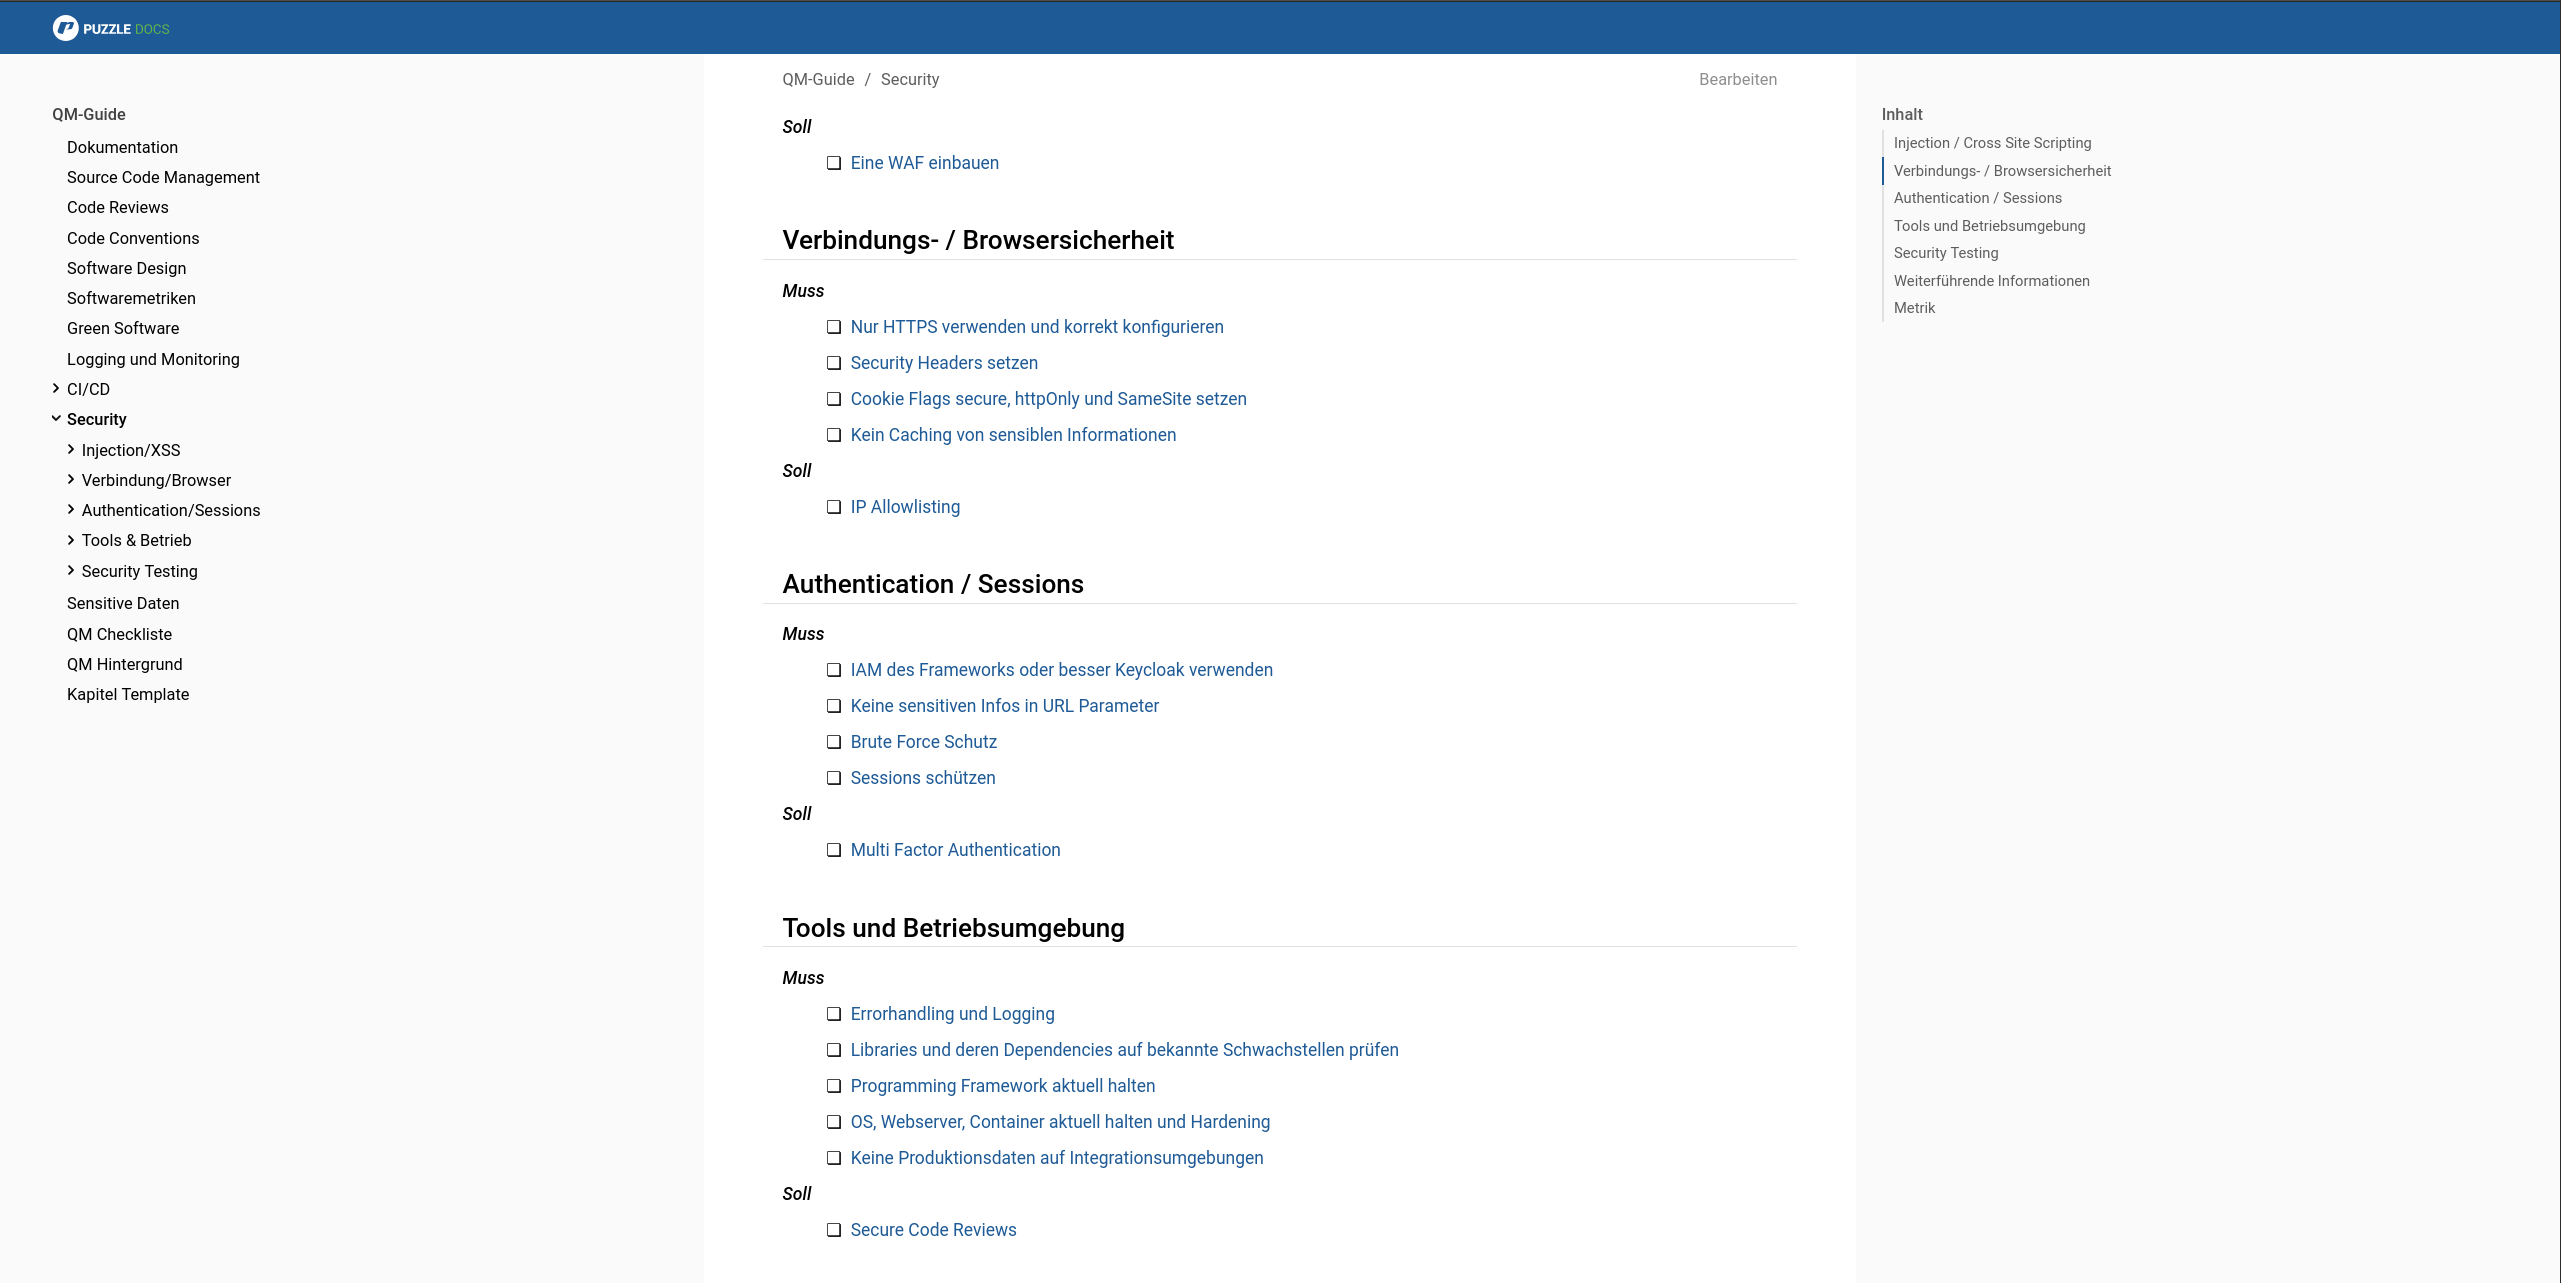
\includegraphics[width=1\textwidth,]{security_conventions_2.png}}
    \caption{Puzzle ITC security conventions 2/3 }
    \end{figure}  
\begin{figure}[h]
    \centering
    \fbox{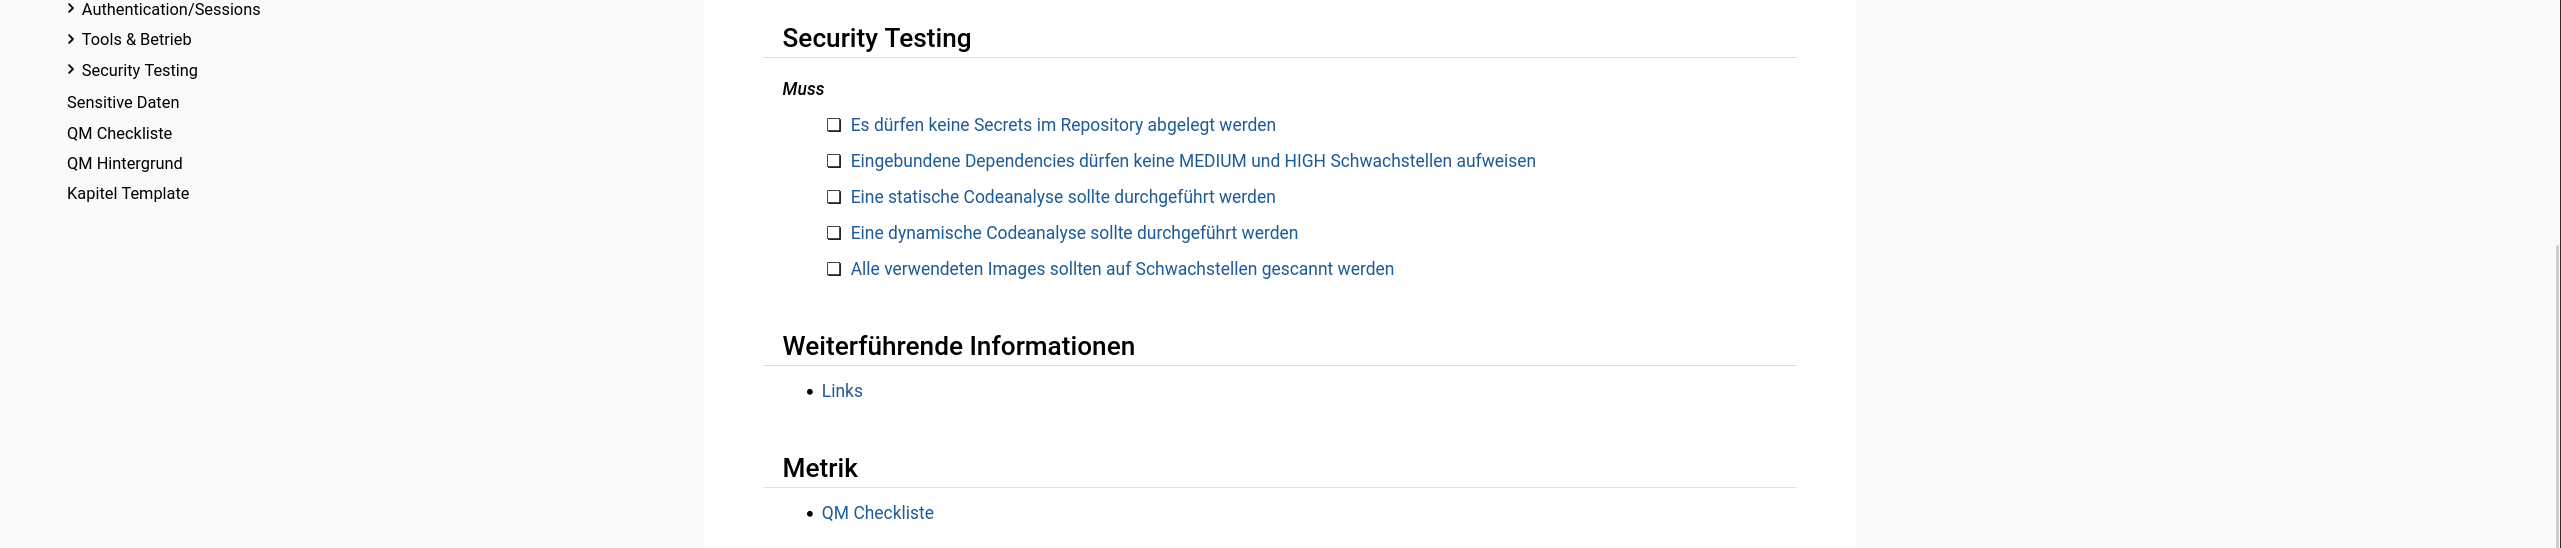
\includegraphics[width=1\textwidth,]{security_conventions_3.png}}
    \caption{Puzzle ITC security conventions 3/3}
    \end{figure}  

\section{Datenschutzkonzept}
\label{sec:datsec}





